\documentclass[a4paper,11pt]{article}
\input{/home/tof/Documents/Cozy/latex-include/preambule_doc.tex}
\input{/home/tof/Documents/Cozy/latex-include/preambule_commun.tex}
\newcommand{\showprof}{show them}  % comment this line if you don't want to see todo environment
\setlength{\fboxrule}{0.8pt}
\fancyhead[L]{\fbox{\Large{\textbf{Algo 10}}}}
\fancyhead[C]{\textbf{Exercices arbre binaire de recherche}}
\newdate{madate}{10}{09}{2020}
%\fancyhead[R]{\displaydate{madate}} %\today
\fancyhead[R]{Terminale - NSI}
\fancyfoot[L]{\vspace{1mm}Christophe Viroulaud}
\AtEndDocument{\label{lastpage}}
\fancyfoot[C]{\textbf{Page \thepage/\pageref{lastpage}}}
\fancyfoot[R]{\includegraphics[width=2cm,align=t]{/home/tof/Documents/Cozy/latex-include/cc.png}}

\begin{document}
\begin{exo}
    Donner tous les ABR formés de trois nœuds contenant les entiers 1, 2, 3.
\end{exo}
\begin{exo}
    \begin{center}
        \begin{tikzpicture}
            \node[draw] (A) at (1,0) {20};
            \node[draw] (B) at (-3,-1) {12};
            \node[draw] (C) at (-5,-2) {5};
            \node[draw] (D) at (-1,-2) {17};
            \node[draw] (F) at (-4,-3) {10};
            \node[draw] (H) at (0,-3) {19};
            \node[draw] (I) at (4,-1) {24};
            \node[draw] (J) at (2,-2) {22};

            \draw (A) -- (B);
            \draw (C) -- (B);
            \draw (C) -- (F);
            \draw (D) -- (B);
            \draw (D) -- (H);
            \draw (A) -- (I);
            \draw (J) -- (I);
            \draw [white] (0,-3) -- (0,-4.5);
        \end{tikzpicture}
        \captionof{figure}{Un Arbre Binaire de Recherche (\emph{ABR})}
        \label{arbre}
    \end{center}
    \begin{enumerate}
        \item Compléter cet ABR en insérant dans l'ordre les valeurs 2, 15, 29, 28.
        \item Donner le résultat d'un parcours infixe de cet ABR.
    \end{enumerate}
\end{exo}
\begin{exo}
    \begin{enumerate}
        \item Écrire la classe \textbf{\texttt{Noeud}} et son constructeur. Ce dernier possédera trois attributs:
              \begin{itemize}
                  \item l'entier \textbf{\texttt{valeur}} initialisé par un paramètre \textbf{\texttt{v}},
                  \item le nœud \textbf{\texttt{gauche}} initialisé à \textbf{\texttt{None}},
                  \item le nœud \textbf{\texttt{droit}} initialisé à \textbf{\texttt{None}}.
              \end{itemize}
        \item Créer une instance \textbf{\texttt{arbre}} de la classe \textbf{\texttt{Noeud}} avec l'argument \textbf{\texttt{13}}.
              \begin{center}
                  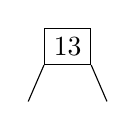
\begin{tikzpicture}
                      \node[draw] (B) at (2,0) {13};

                      \draw (B.south west) -- (1.5,-0.7);
                      \draw (B.south east) -- (2.5,-0.7);
                  \end{tikzpicture}
                  \captionof{figure}{Racine de l'arbre binaire de recherche}
                  \label{noeud}
              \end{center}
        \item Écrire la méthode \textbf{\texttt{inserer(self, v: int) $\rightarrow$ None}} de la classe \textbf{\texttt{Noeud}} qui insère récursivement \textbf{\texttt{v}} dans le sous-arbre gauche ou droit.
        \item Insérer 10 entiers aléatoires distincts dans \textbf{\texttt{arbre}}.
        \item Écrire la méthode \textbf{\texttt{rechercher(self, v: int) $\rightarrow$ bool}} de la classe \textbf{\texttt{Noeud}} qui vérifie récursivement si \textbf{\texttt{v}} est présent dans l'arbre.
        \item Tester la méthode dans les deux cas de figures (valeur trouvée ou non).
        \item Écrire la méthode itérative \textbf{\texttt{minimum(self) $\rightarrow$ int}} qui renvoie la valeur minimale de l'arbre.
        \item Écrire la version récursive de \textbf{\texttt{minimum}}.
        \item Écrire la méthode récursive \textbf{\texttt{infixe(self, noeud: object, parcours: list) $\rightarrow$ None}} qui effectue un parcours infixe dans \textbf{\texttt{arbre}}.
    \end{enumerate}
\end{exo}
\begin{exo}
D'après épreuve pratique BAC 2020\\
Dans cet exercice, un arbre binaire de caractères est stocké sous la forme d’un dictionnaire où les clefs sont les caractères des nœuds de l’arbre et les valeurs, pour
chaque clef, la liste des caractères des fils gauche et droit du nœud.
\begin{center}
    \begin{tikzpicture}
        \node[draw] (A) at (1,0) {F};
        \node[draw] (B) at (-3,-1) {B};
        \node[draw] (C) at (-5,-2) {A};
        \node[draw] (D) at (-1,-2) {D};
        \node[draw] (H) at (0,-3) {E};
        \node[draw] (I) at (4,-1) {G};
        \node[draw] (L) at (-2,-3) {C};
        \node[draw] (M) at (5,-2) {I};
        \node[draw] (N) at (6,-3) {H};

        \draw (A) -- (B);
        \draw (C) -- (B);
        \draw (D) -- (B);
        \draw (D) -- (H);
        \draw (A) -- (I);
        \draw (L) -- (D);
        \draw (M) -- (I);
        \draw (M) -- (N);
    \end{tikzpicture}
\end{center}
Par exemple, l'arbre ci-dessus est stocké dans:
\begin{center}
\begin{lstlisting}[language=Python  , xleftmargin=2em, xrightmargin=2em]
a = {'F':['B','G'], 'B':['A','D'], 'A':['',''], 'D':['C','E'], 'C':['',''], 'E':['',''], 'G':['','I'], 'I':['','H'], 'H':['','']}
\end{lstlisting}
\end{center}
Écrire une fonction récursive \texttt{\textbf{taille}} prenant en paramètres un arbre binaire arbre
sous la forme d’un dictionnaire et un caractère lettre qui est la valeur du sommet de l’arbre, et qui renvoie la taille de l’arbre à savoir le nombre total de nœud.\\
On pourra distinguer les 4 cas où les deux « fils » du nœud sont '', le fils gauche seulement est '', le fils droit seulement est '', aucun des deux fils n’est ''.
\begin{center}
\begin{lstlisting}[language=Python  , xleftmargin=2em, xrightmargin=2em]
>>> taille(a, ’F’)
9
\end{lstlisting}
\captionof{code}{Exemple}
\label{CODE}
\end{center}
\end{exo}
\end{document}